%%%%                          %%%%
%%%% FUNDAMENTOS TECNOLÓGICOS %%%%
%%%%                          %%%%

\chapter{Fundamentos tecnológicos}
\label{chap:fundamentos-tecnologicos}

El objetivo de este capítulo es sentar las bases tenológicas y teóricas sobre las que se ha llevado a cabo el proyecto.

\section{¿El formato PDF? Estructura de un PDF}

Son tres las tecnologías base que componen el formato PDF:

\begin{itemize}
	\item Los PDF se escriben como un subconjunto del lenguaje de programación PostScript.
	\item Un sistema para incrustar y reemplazar fuentes tipográficas.
	\item Un sistema estructurado de almacenamiento para unir todos los elementos en un único fichero.
\end{itemize}

Otros elementos deben incluirse en formato \acrfull{cos}. Un árbol cos contiene objetos de los siguientes tipos:

\begin{enumerate}
	\item Boolean values
	\item Numbers
	\item Strings
	\item Arrays
	\item Dictionaries
	\item Streams
	\item Null object
\end{enumerate}

Relaciones entre los espacios de coordenadas de un PDF:

\begin{figure}[hp!]
	\centering
	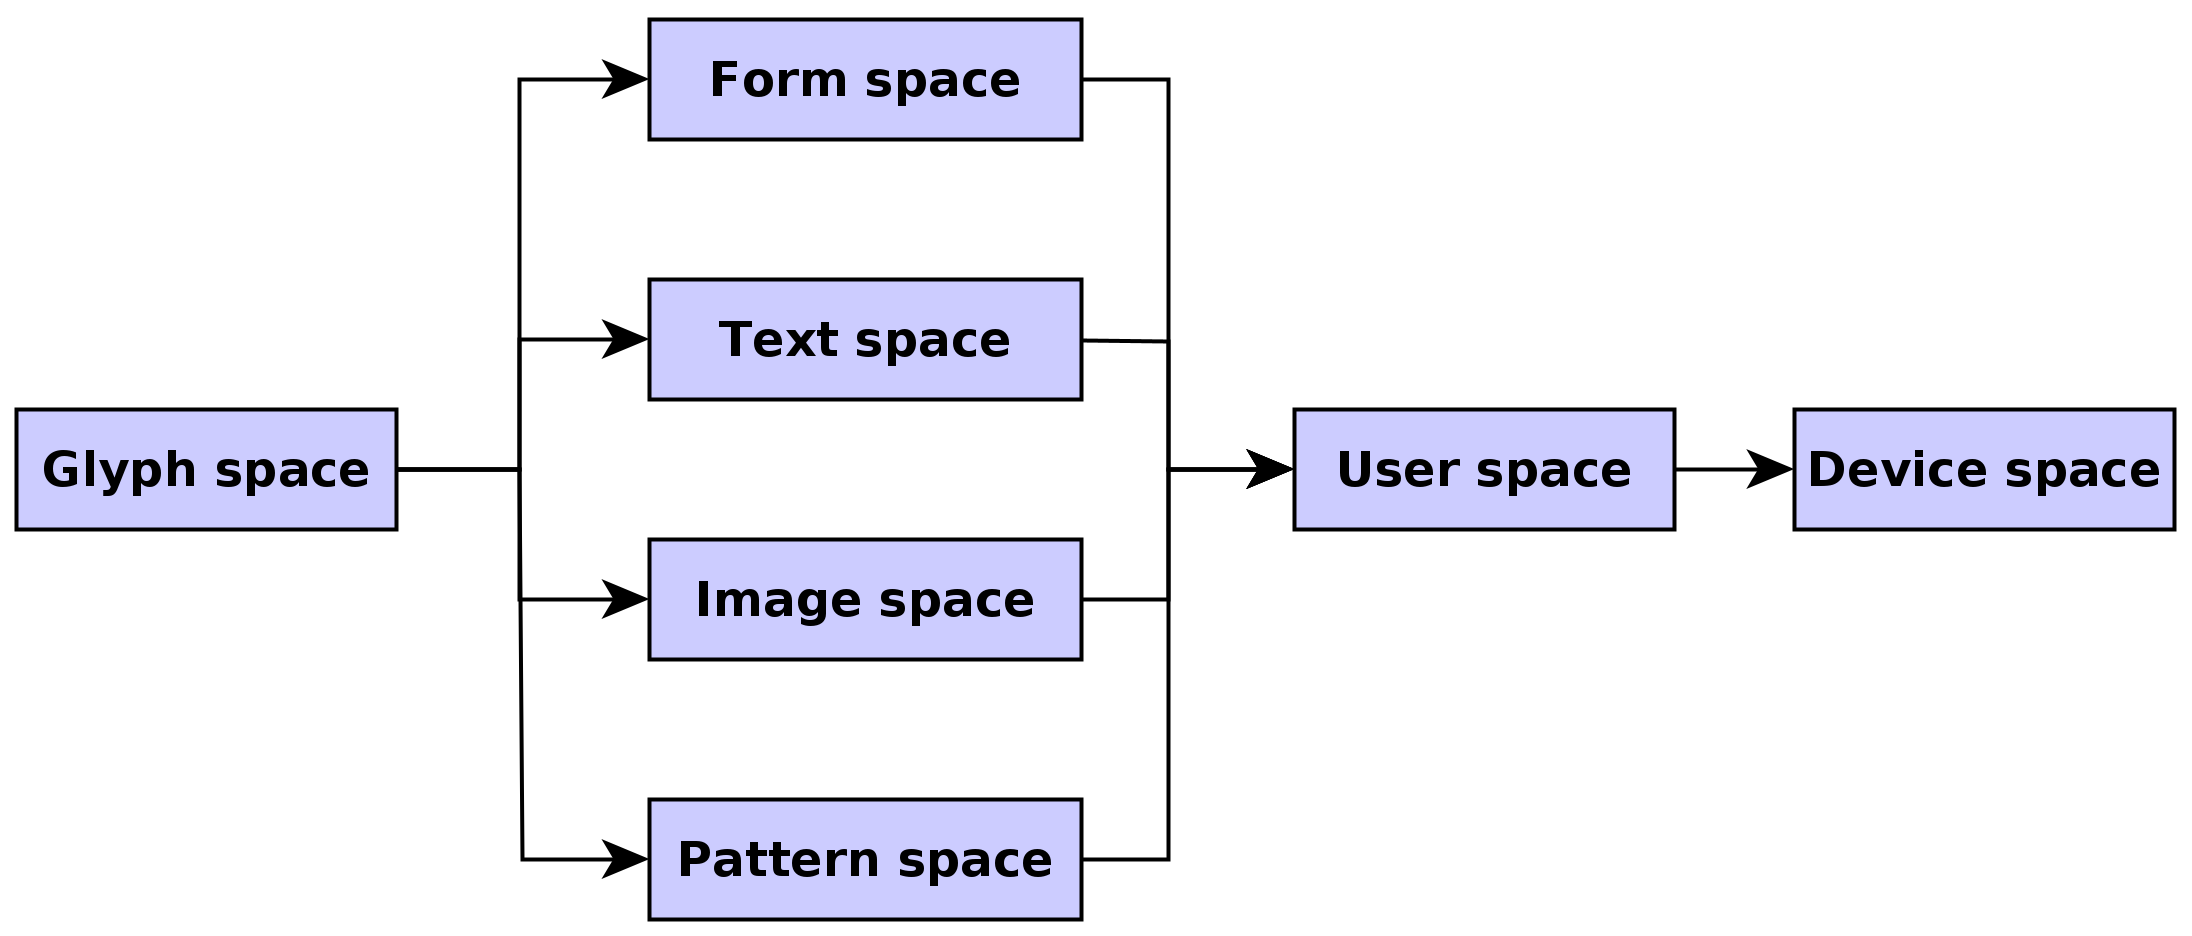
\includegraphics[width=11cm]{imaxes/espacios-coordenadas.png}
\end{figure}

¿Por qué el formato PDF almacena las coordenadas de las regiones?

\section{Información de coordenadas en documentos}
\subsection{El microformato HOCR y otras alternativas}
\subsection{Pdftotext e información de bounding box}

\section{OCR con Tesseract}

Existen numerosas herramientas para llevar a cabo Reconocimiento Óptico de Caracteres. Entre ellas destaca Tesseract. Tesseract es un \emph{engine} de código abierto y desarrollado inicialmente por Hewlett Packard entre los años 1985 y 1995. Después de un periodo sin actividad, en el 2006 el proyecto fue recuperado por Google, que lo mantiene desde entonces.

Hoy en día tiene soporte para más de cien idiomas y la red neuronal que utiliza \footnote{Desde la versión 4, Tesseract utiliza una red LSTM. Esta es una red de tipo Red Neuronal Recurrente} puede ser entrenada para casos específicos si fuese necesario. Existe una amplia documentación en la web oficial, además, numerosos tutoriales en la red permiten familiarizarse con la herramienta al tratarse de un proyecto bien conocido y de larga trayectoria.

Se puede obtener como salida el texto reconocido y también la información de las coordenada, sobre el documento, de las palabras detectadas. Esta información resulta fundamental para poder aplicar las plantillas utilizadas este proyecto. 

\section{Transformada de Hough}

La transformada de Hough es una técnica de visión por computador utilizada para detectar figuras parametrizables, tales como líneas o círculos. El algoritmo parte de una imagen binaria que representa los bordes encontrados por una detector de bordes. A continuación se calculan todas las posibles líneas que podrían pasar por cada punto y se lleva a cabo una votación. Se seleccionan las líneas más votadas, entre todas las detectadas.

Este algoritmo proporciona una manera automática de localizar los bordes entre líneas de las tablas de muchos documentos y evita la necesidad de incorporar dicha información a las plantillas de forma manual. Se utiliza la implementación incluida en la librería OpenCV.

\section{GNU Make}
\section{Flex y Bison}
\section{Ansible}
\section{Docker}


%% Valorar si mencionar otras herramientas como:
% Extracción de texto: Apache PDFBox, pdftotext
% OCR: Tesseract
% Pretty print de JSON: jq
